% !TeX program = lualatex
% !TeX encoding = utf8
% !BIB program = biber
% !TeX spellcheck = uk_UA

\documentclass{mathreport}
% ------------------------------------------------------------------------------------------------------------
% Add Additional Packages
% ------------------------------------------------------------------------------------------------------------

\renewcommand{\theequation}{\arabic{subsection}.\arabic{equation}}
\renewcommand{\thesubsection}{\arabic{subsection}}

\usepackage{bbm} % for using indicator \mathbbm{1}

% reset equation numbering after each subsection
\counterwithin*{equation}{subsection}

% set page background color (dark read mode)
% \pagecolor[rgb]{0.118,0.118,0.118}
% \color[rgb]{0.8,0.8,0.8}

\begin{document}

\ReportPreamble{Лабораторна робота №2 -- №3}
\ReportName{Задача динамічного деформування твердого тіла}
\ReportSubject{Чисельні методи математичної фізики}

\AuthorInfo{Студент 5 курсу, групи КМ-31мн,}
\AuthorName{Цибульник Антон Владиславович}

\SupervisorInfo{Професор кафедри ПМА,}
\SupervisorName{Ориняк Ігор Володимирович}

% warning: in order to fit the text in the very right side of a page, set the longest label
\TheLongestLabel{Цибульник Антон Владиславович}

\import{Title/}{title}

\tableofcontents

\newpage

\section{Постановка задачі}
% \addcontentsline{toc}{section}{Постановка задачі}

У лабораторній роботі розглядається задача динамічного деформування балки в часі. Для балки, що згинається, кожна точка $s$ балки довжиною $2L$ в кожен момент часу $t$ характеризується чотирма параметрами: переміщенням $W(s,t)$, кутом згинання $\theta(s,t)$, згинальним моментом $M(s,t)$ та внутрішньою поперечною силою $Q(s,t)$. Відтак, деформуванню балки відповідатиме така система диференціальних рівнянь:
\begin{align}\label{eq: initial d.e.}
    \frac{\partial W(s,t)}{\partial s} = \theta(s,t), &&  \frac{\partial\theta(s,t)}{\partial s} = M(s,t), && \frac{\partial M(s,t)}{\partial s} = Q(s,t), && \frac{\partial Q(s,t)}{\partial s} = \alpha(s,t),
\end{align}
де в рамках потавленої задачі розподілена сила $\alpha(s,t)$ має дві складові різної природи: силу інерції, направлену в протилежний до напрямку переміщення бік
\begin{equation}\label{eq: inertia force}
    p_{in}(s,t) = -\frac{\partial^2 W(s,t)}{\partial t^2},
\end{equation}
та зовнішню силу
\begin{equation}\label{eq: external force}
    p_{ex}(s,t) = p_0\, \delta(s-L/2) \cos{\eta t},
\end{equation}
де $p_0$ є константою, $\delta(s-s_0)$ є дельта-функцією Дірака, яка задає зосереджену силу в точці $s_0=L/2$, а параметр $\eta$ є частотою дії зовнішньої сили. 

Зауважимо, що сталі характеристики системи, такі як модуль пружності $E$, характеристика геометрії січення $J$ та площа перерізу балки $S$ покладені одниці. Також зазначимо, що дельта-функція Дірака $\delta(s-s_0)$ приймає нульове значення усюди, окрім околу точки $s_0$, де її значення сягає нескінченності:
\begin{align}\label{eq: delta Dirac}
    \delta(s-s_0)=
    \begin{cases*}
        0, & $s \neq s_0$ \\
        \infty, & $s=s_0$ \\
    \end{cases*},
\end{align}
та, крім того, в загальному випадку дельта-функція Дірака $\delta(s)$ володіє такими властивостями на області дії $D:$
\begin{align}
    & \int\limits_{D}\delta(s)\,ds = 1 \label{eq: delta Dirac feature 1} \\
    & \int\limits_{D}\delta(s-s_0)f(s)\,ds = f(s_0) \label{eq: delta Dirac feature 2}
\end{align}

Отже, звівши систему чотирьох рівнянь~\eqref{eq: initial d.e.} до одного рівняння четвертого ступеня,  моделювання динамічного деформування балки описуватиметься таким диференціальним співвідношенням:
\begin{equation}\label{eq: united d.e.}
    \frac{\partial^4 W(s,t)}{\partial s^4} + \frac{\partial^2 W(s,t)}{\partial t^2} = p_{ex}(s,t) = p_0\,\delta(s-L/2) \cos{\eta t}
\end{equation}
із чотирма граничними умовами
\begin{align}\label{eq: edge conditions}
    W(0,t)=0, && W(2L,t)=0, && \frac{\partial^2W(0,t)}{\partial s^2}=0, && \frac{\partial^2W(2L,t)}{\partial s^2}=0
\end{align}

Наостанок, балка, яка підлягає деформуванню, згідно з умовами задачі має особливість~--- проміжну опору в точці $L$. Тож на додачу до граничних умов~\eqref{eq: edge conditions} отримуємо обмеження виду
\begin{align}\label{eq: central condition}
    W(L,t)=0
\end{align}

У подальших викладках буде розглянуто пошук точного аналітичного розв'язку за методом початкових параметрів (МПП) й наближеного аналітичного розв'язку за методом зважених залишків (МЗЗ) для системи рівнянь~\eqref{eq: united d.e.} у випадку відсутності дії зовнішнього навантаження (однорідне рівняння деформації) та у випадку наявного зовнішнього навантаження (неоднорідне рівняння деформації).

\section{Ідея методу початкових параметрів (МПП)}

Метод початкових параметрів розглядає довільну систему як такі сутності: елементи; межі між елементами (кінці, вузли), де відбувається спряження дотичних елементів; границі всієї системи. При цьому для системи вводиться поняття потужності $N$ --- кількості параметрів, які визначають стан системи в кожній його точці $s$. Виокремлення окреслених вище сутностей системи відбувається поетапно разом із такими супутніми процедурами:

\begin{enumerate}
    \item Система дробиться на декілька окремих ділянок (елементів), і кожна така ділянка нумерується відповідним чином. Після цього визначаються вхідні та вихідні краї кожного елемента, а також вузли --- точки одночасного дотику декількох елементів. Іншими словами, відбувається організація обходу по елементах системи;
    \item Нумерація невідомих змінних (параметрів) на кожному із двох країв кожного елемента системи;
    \item Складання так званих рівнянь зв’язку для кожного елемента. Ці рівняння зв’язують параметри в кінцевій точці елемента зі значеннями в точці початку елемента. Рівняння зв'язку випливають з фізичних чи геометричних властивостей кожного елемента та системи в цілому;
    \item Складання рівнянь спряження в кожному вузлі системи;
    \item Складання рівнянь, що відповідають граничним умовам системи.
\end{enumerate}

Для системи потужності $N$, що складається з $K$ елементів, кількість невідомих параметрів системи складає $2KN$, адже для кожного елемента визначено невідомі змінні (параметри) на його початку та в його кінці. Відповідно, кількість складених рівнянь згідно з методом початкових параметрів має бути $2KN$.  

\section{Ідея методу зважених залишків (МЗЗ)}

Метод зважених залишків оперує рівнянням вигляду
\begin{equation}\label{eq: G(y) = f(x)}
    G(y) = f(x),
\end{equation}
де $G(y)$~--- деякий заданий лінійний диференціальний оператор над функцією $y(x)$, а $f(x)$ у правій частині є певним зовнішнім навантаженням (дією зовнішніх сил). Припускається, що функція $y(x)$ має форму суми $M$ так званих базових функцій $\phi_i(x)$, помножених на невідомі коефіцієнти $a_i$:
\begin{equation}\label{eq: y(x) approximation}
    y(x) = \sum\limits_{i=1}^{M} a_i\phi_i(x)
\end{equation}

Зауважимо, що перелік базових функцій задається так, щоб задовольнити нульові граничні умови задачі. Отже, оскільки вигляд~\eqref{eq: y(x) approximation}~--- лише наближення невідомої функції $y(x)$, вводиться поняття залишку диференціального оператора:
\begin{equation}\label{eq: R(x) residual}
    R(x) = \sum\limits_{i=1}^{M} a_i G\bigl( \phi_i(x) \bigr) - f(x)
\end{equation}

Мета методу полягає у мінімізації утвореного залишку $R(x)$ шляхом пошуку оптимальних значень коефіцієнтів $a_i$ через почергову процедуру <<зваження>> з кожною базовою функцією $\phi_i(x)$:
\begin{equation}\label{eq: R(x) minimizing}
    \int\limits_{\mathbb{R}} R(x)\, \phi_i(x)\, dx = 0,\ i=\overline{1,M}
\end{equation}

Таким чином, кількість рівнянь~\eqref{eq: R(x) minimizing} дорівнює кількості невідомих коефіцієнтів $a_i$, що дозволяє розв'язати утворену систему рівнянь та отримати наближене аналітичне рішення згідно з припущенням~\eqref{eq: y(x) approximation}.

\section{Рішення однорідного рівняння деформації}

\subsection*{Деталізація поставленої задачі за МПП}
\addcontentsline{toc}{subsection}{Деталізація поставленої задачі за МПП}
\label{section: TMM detalization}

Розглянемо покроково кожен етап МПП в рамках задачі динамічного деформування тіла на площині. Перш за все, з огляду на поставлену задачу~\eqref{eq: initial d.e.}, потужність системи складає $N=4$. Організацію обходу по елементах системи виконаємо таким чином: визначимо $K=2$ елементи та, відповідно, один вузол у точці опори $L$~(Рис.~\ref{pic: beam}).

\vspace{0.4cm}
\begin{figure}[H]\centering
    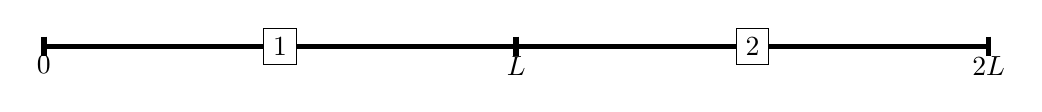
\begin{tikzpicture}
    \pgfmathsetmacro{\L}{6}
    \pgfmathsetmacro{\ticklen}{0.125}

    % element labels
    \node[draw,rectangle] (P1) at (-\L/2,0) {1};
    \node[draw,rectangle] (P2) at (\L/2,0) {2};

    % main line (beam)
    \draw[line width=2pt] (-\L,0) -- (P1) -- (P2) -- (\L,0);

    % ticks
    \draw[line width=2pt] (-\L,\ticklen) -- (-\L,-\ticklen);
    \draw[line width=2pt] (0,\ticklen) -- (0,-\ticklen);
    \draw[line width=2pt] (\L,\ticklen) -- (\L,-\ticklen);

    % labels
    \coordinate[label=below:{$0$}] (E1) at (-\L,0);
    \coordinate[label=below:{$L$}] (E2) at (0,0);
    \coordinate[label=below:{$2L$}] (E3) at (\L,0);
\end{tikzpicture}
    \caption{Балка довжиною $2L$ як система двох елементів}
    \label{pic: beam}
\end{figure}

Дію зовнішнього навантаження~\eqref{eq: external force} на систему~\eqref{eq: united d.e.} позначено на Рис.~\ref{pic: beam with forces}.

\vspace{0.4cm}
\begin{figure}[H]\centering
    \begin{tikzpicture}
    \pgfmathsetmacro{\L}{6}
    \pgfmathsetmacro{\ticklen}{0.125}

    % element labels
    % \node[draw,rectangle] (P1) at (-\L/2,0) {1};
    % \node[draw,rectangle] (P2) at (\L/2,0) {2};

    % main line (beam)
    \draw[line width=2pt] (-\L,0) -- (\L,0);

    % ticks
    \draw[line width=2pt] (-\L,\ticklen) -- (-\L,-\ticklen);
    \draw[line width=2pt] (-\L/2,\ticklen) -- (-\L/2,-\ticklen);
    \draw[line width=2pt] (0,\ticklen) -- (0,-\ticklen);
    \draw[line width=2pt] (\L,\ticklen) -- (\L,-\ticklen);

    % labels
    \coordinate[label=below:{$0$}] (E1) at (-\L,0);
    \coordinate[label=above:{$L/2$}] (E2) at (-\L/2,0);
    \coordinate[label=below:{$L$}] (E3) at (0,0);
    \coordinate[label=below:{$2L$}] (E4) at (\L,0);

    % force arrows
    \draw[-{Stealth[scale=1.2]},shorten >= 7.5pt,line width=1.25pt] 
        (-\L/2,-1.4) -- (E2) node[at start,below] {$p_0\,\delta(s-L/2)\cos{\eta t}$};
\end{tikzpicture}
    \caption{Балка під дією зосередженої сили}
    \label{pic: beam with forces}
\end{figure}

Складемо нумерацію невідомих параметрів переміщення $W(s,t)$, кута згинання $\theta(s,t)$, згинального моменту $M(s,t)$ та внутрішньої поперечної сили $Q(s,t)$ на початку та в кінці кожного елемента. В результаті отримаємо $2KN=16$ змінних, зображених у Табл.~\ref{table: variables numeration TMM}.

\vspace{0.4cm}
\begin{table}[H]\centering
    \begin{tblr}{
            hlines={1pt,solid}, 
            vlines={1pt,solid},
            hline{4-6}={1-5}{0pt},
            colspec={X[c]X[c]X[c]X[c]X[c]},
            cell{1}{1}={r=2,c=1}{c},
            cell{1}{2}={r=1,c=2}{c},
            cell{1}{4}={r=1,c=2}{c},
            row{3-6}={mode=math},
        }
        
                    & Елемент <<$1$>> & & Елемент <<$2$>> &  \\
                    & Початок & Кінець  & Початок & Кінець   \\
        W(s,t)      & x_{1}   & x_{5}   & x_{9}   & x_{13}   \\
        \theta(s,t) & x_{2}   & x_{6}   & x_{10}  & x_{14}   \\
        M(s,t)      & x_{3}   & x_{7}   & x_{11}  & x_{15}   \\
        Q(s,t)      & x_{4}   & x_{8}   & x_{12}  & x_{16}   \\

    \end{tblr}
    \caption{Нумерація невідомих параметрів системи}
    \label{table: variables numeration TMM}
\end{table}

\subsubsection*{Складання рівнянь системи}
\addcontentsline{toc}{subsubsection}{Складання рівнянь системи}

Пошук розв'язку задачі динамічного деформування тіла на площині при відсутній дії зовнішнього навантаження~$p_{ex}(s,t)=0$ описуватиметься згідно з~\eqref{eq: united d.e.} однорідним рівнянням виду
\begin{equation}\label{eq: homogeneous d.e.}
    \frac{\partial^4 W(s,t)}{\partial s^4} + \frac{\partial^2 W(s,t)}{\partial t^2} = 0
\end{equation}

Для визначення рівнянь зв'язку на елементі <<$1$>> та елементі <<$2$>>~(Рис.~\ref{pic: beam}) використаємо метод Фур'є, який ще називають методом розділення змінних. Метод полягає у представленні невідомої функції $W(s,t)$ у вигляді добутку функції кординати~$W(s)$ та функції часу~$T(t):$ 
\begin{equation}\label{eq: fourier method}
    W(s,t) = W(s)\,T(t)
\end{equation}

Підставимо цей вираз у рівняння~\eqref{eq: homogeneous d.e.}:
\begin{equation}\label{eq: homogeneous fourier d.e.}
    \frac{d^4 W(s)}{d s^4}\,T(t) + \frac{d^2 T(t)}{d t^2}\,W(s) = 0
\end{equation}

Відтак, виконавши еквівалентні перетворення, отримаємо
\begin{equation}\label{eq: edited homogeneous fourier d.e.}
    \frac{W^{(4)}(s)}{W(s)} + \frac{T''(t)}{T(t)} = 0 \ \Longrightarrow \ \frac{W^{(4)}(s)}{W(s)} = - \frac{T''(t)}{T(t)} = \omega^2,
\end{equation}
де введемо константу $\omega$, яка матиме зміст власної частоти розв'язку однорідного диференціального рівняння~\eqref{eq: homogeneous d.e.}. 

Згідно з умовами задачі, функція часу $T(t)$ розглядатиметься лише як частинний розв'язок, який задовільняє відповідному диференціальному рівнянню~\eqref{eq: edited homogeneous fourier d.e.}, тож в межах лабораторної роботи покладемо
\begin{equation}\label{eq: T(t) assumption}
    T(t) = \cos{\omega t},
\end{equation}
при цьому зауважимо, що при підстановці цього частинного рішення у рівняння~\eqref{eq: homogeneous fourier d.e.} функціональна залежність від часу скорочується. Таким чином, керівним розв'язком системи стає функція $W(s)$ відносно координати. 

Власне кажучи, наступним кроком перейдемо до розгляду розв'язку рівняння~\eqref{eq: edited homogeneous fourier d.e.} відносно координати, позначивши $k_{\omega}^4=\omega^2:$
\begin{equation}\label{eq: W(s) homogeneous fourier d.e.}
    W^{(4)}(s) - k_{\omega}^4 W(s) = 0
\end{equation}

\newpage
Тоді, виконавши заміну $W(s)=e^{\lambda s}$, знайдемо розв'язок лінійного однорідного диференціального рівняння четвертого ступеня зі сталими коефіцієнтами за методологією пошуку власних значень $\left( \lambda_j \right)_{j=\overline{1,4}}$ відповідного характеристичного рівняння:
\begin{equation}\label{eq: eigenvalues}
    \lambda_{1,2,3,4} = -k_{\omega},\, k_{\omega},\, -ik_{\omega},\, ik_{\omega},
\end{equation} 
а відтак розв'язок, відповідно, матиме вигляд:
\begin{equation}\label{eq: solution of homogeneous d.e.}
    W(s) = \sum\limits_{j=1}^{4} C_j e^{\lambda_j s} = C_1e^{-k_{\omega} s} + C_2e^{k_{\omega} s} + C_3e^{-ik_{\omega} s} + C_4e^{ik_{\omega} s},
\end{equation} 
де, враховуючи тригонометричні співвідношення
\begin{align}\label{eq: trigonometric ratios}
    \cosh{s} = \frac{e^{s}+e^{-s}}{2}, \qquad \sinh{s} = \frac{e^{s}-e^{-s}}{2}, \\
    \cos{s} = \frac{e^{is}+e^{-is}}{2}, \qquad \sin{s} = \frac{e^{is}-e^{-is}}{2},
\end{align}
остаточний розв'язок рівняння~\eqref{eq: W(s) homogeneous fourier d.e.} матиме вид:
\begin{equation}\label{eq: final solution of homogeneous d.e.}
    W(s) = C_1\cosh{k_{\omega} s} + C_2\sinh{k_{\omega} s} + C_3\cos{k_{\omega} s} + C_4\sin{k_{\omega} s}
\end{equation}

В рамках методу МПП коефіцієнти $C_1$, $C_2$, $C_3$, $C_4$ визначатимуться через задовільнення локальних граничних умов на кожній ділянці системи $s \in [0,L]$ при фіксованому~$t:$ 
\begin{align}\label{eq: TMM initial conditions, element 1}
    W(0)=W_0, && \frac{dW(0)}{ds}=\theta_0, && \frac{d^2W(0)}{ds^2}=M_0, && \frac{d^3W(0)}{ds^3}=Q_0,
\end{align}
відтак матимемо
\begin{align}\label{eq: A1, A2, A3, A4 for element 1}
    C_1=\frac{W_0}{2} + \frac{M_0}{2k_{\omega}^2}, 
    \qquad C_2=\frac{\theta_0}{2k_{\omega}} + \frac{Q_0}{2k_{\omega}^3}, \\
    C_3=\frac{W_0}{2} - \frac{M_0}{2k_{\omega}^2},
    \qquad C_4=\frac{\theta_0}{2k_{\omega}} - \frac{Q_0}{2k_{\omega}^3},
\end{align}
а отже, згрупувавши складові функції $W(s)$ навколо значень невідомих параметрів на початку елемента, отримуємо розв'язок однорідного рівняння деформації відносно координати:
\begin{equation}\label{eq: W(s) for element 1}
    W(s) = W_0 K_1(s) + \theta_0 K_2(s) + M_0 K_3(s) + Q_0 K_4(s),
\end{equation}
де нижче наведені функції є так званими узагальненими функціями Крилова:
\begin{align}\label{eq: Krylov for element 1}
    & K_1(s) = \tfrac{1}{2} (\cosh{k_{\omega} s} + \cos{k_{\omega} s}) \\
    & K_2(s) = \tfrac{1}{2k_{\omega}} (\sinh{k_{\omega} s} + \sin{k_{\omega} s}) \\
    & K_3(s) = \tfrac{1}{2k_{\omega}^2} (\cosh{k_{\omega} s} - \cos{k_{\omega} s}) \\
    & K_4(s) = \tfrac{1}{2k_{\omega}^3} (\sinh{k_{\omega} s} - \sin{k_{\omega} s})
\end{align}

Таким чином, взявши першу похідну від переміщення~\eqref{eq: W(s) for element 1} для кута згинання, другу похідну для згинального моменту та третю похідну для внутрішньої поперечної сили, отримуємо відповідну систему рівнянь зв'язку в локальних координатах на кожному елементі системи, враховуючи відповідні значення початкових параметрів.

Наприклад, на елементі <<$1$>> (Рис.~\ref{pic: beam}) початкові параметри позначимо як $W_0$, $\theta_0$, $M_0$ та $Q_0$, а отже в межах локальних координат $s \in [0,L]$ матимемо такі рівняння зв'язку:
\begin{align}\label{eq: field equations for element 1}
    & W(s) = W_0 K_1(s) + \theta_0 K_2(s) + M_0 K_3(s) + Q_0 K_4(s) \\
    & \theta(s) = k_{\omega}^4 W_0 K_4(s) + \theta_0 K_1(s) + M_0 K_2(s) + Q_0 K_3(s) \\
    & M(s) = k_{\omega}^4 W_0 K_3(s) + k_{\omega}^4 \theta_0 K_4(s) + M_0 K_1(s) + Q_0 K_2(s) \\
    & Q(s) = k_{\omega}^4 W_0 K_2(s) + k_{\omega}^4 \theta_0 K_3(s) + k_{\omega}^4 M_0 K_4(s) + Q_0 K_1(s)
\end{align}

Або у матричному вигляді:
\begin{equation}\label{eq: matrix field equations for element 1}
    \begin{pmatrix}
        W(s)      \\
        \theta(s) \\
        M(s)      \\
        Q(s)      \\
    \end{pmatrix} =
    \begin{pmatrix}
        K_1(s)          & K_2(s)          & K_3(s)          & K_4(s) \\
        k_{\omega}^4 K_4(s) & K_1(s)          & K_2(s)          & K_3(s) \\
        k_{\omega}^4 K_3(s) & k_{\omega}^4 K_4(s) & K_1(s)          & K_2(s) \\
        k_{\omega}^4 K_2(s) & k_{\omega}^4 K_3(s) & k_{\omega}^4 K_4(s) & K_1(s) \\
    \end{pmatrix}
    \begin{pmatrix}
        W_0      \\
        \theta_0 \\
        M_0      \\
        Q_0      \\
    \end{pmatrix}
\end{equation} 

Аналогічними міркуваннями в межах локальних координат $s \in [0,L]$ на елементі <<$2$>> з початковими параметрами $W_L$, $\theta_L$, $M_L$ та $Q_L$ матимемо такі рівняння зв'язку у матричному вигляді:
\begin{equation}\label{eq: matrix field equations for element 2}
    \begin{pmatrix}
        W(s)      \\
        \theta(s) \\
        M(s)      \\
        Q(s)      \\
    \end{pmatrix} =
    \begin{pmatrix}
        K_1(s)          & K_2(s)          & K_3(s)          & K_4(s) \\
        k_{\omega}^4 K_4(s) & K_1(s)          & K_2(s)          & K_3(s) \\
        k_{\omega}^4 K_3(s) & k_{\omega}^4 K_4(s) & K_1(s)          & K_2(s) \\
        k_{\omega}^4 K_2(s) & k_{\omega}^4 K_3(s) & k_{\omega}^4 K_4(s) & K_1(s) \\
    \end{pmatrix}
    \begin{pmatrix}
        W_L      \\
        \theta_L \\
        M_L      \\
        Q_L      \\
    \end{pmatrix}
\end{equation} 

На додачу до вісьмох рівнянь зв'язку \eqref{eq: matrix field equations for element 1} та \eqref{eq: matrix field equations for element 2} введемо чотири рівняння, що відповідають глобальним граничним умовам~\eqref{eq: edge conditions}, та чотири рівняння спряження в точні опори (Табл.~\ref{table: transition equations}). Відтак, матимемо повний комплект із 16 рівнянь для 16 невідомих змінних (Табл.~\ref{table: variables numeration TMM}) системи. 

У складеній системі рівнянь значення власної частоти так і лишається невизначеним. У наступному підрозділі будуть наведені кроки, покликані визначити значення~$\omega$.

\vspace{0.4cm}
\begin{table}[H]\centering
    \begin{tblr}{
            hlines={1pt,solid}, 
            vlines={1pt,solid},
            hline{3-5}={1-3}{0pt},
            colspec={X[c]X[c]X[c]},
            row{2-5}={mode=math},
            row{1}={m}
        }
        
        Граничні рівняння зліва & Рівняння спряження & Граничні рівняння справа \\
                                & x_{9}  = x_{5}     &                          \\
        x_{1} = 0               & x_{10} = x_{6}     & x_{13} = 0               \\
        x_{3} = 0               & x_{11} = x_{7}     & x_{15} = 0               \\
                                & x_{9} = 0          &                          \\

    \end{tblr}
    \caption{Рівняння зв'язку та спряження системи}
    \label{table: transition equations}
\end{table} 

\subsubsection*{Визначення власних частот}
\addcontentsline{toc}{subsubsection}{Визначення власних частот}

Враховуючи граничні умови $x_1=0$ та $x_3=0$ (Табл.~\ref{table: transition equations}), а також умову нульового переміщення в точці опори $x_5=0$, зафіксуємо змінну $x_2$ (значення~$\theta_0$), і тоді згідно з рівнянням зв'язку для переміщення на елементі <<1>>~\eqref{eq: matrix field equations for element 1} матимемо:
\begin{equation}\label{eq: x4}
    x_5 = x_1 K_1(L) + x_2 K_2(L) + x_3 K_3(L) + x_4 K_4(L) \ \Longrightarrow \ x_4 = -\frac{K_2(L)}{K_4(L)}\, x_2
\end{equation}

Відтак маємо змогу визначити значення параметрів в кінці елемента <<1>>:
\begin{align}\label{eq: x6 x7 x8}
    & x_6 = x_2 \left( K_1(L) - K_3(L)\frac{K_2(L)}{K_4(L)} \right) \\
    & x_7 = x_2 \left( k_{\omega}^4 K_4(L) - K_2(L)\frac{K_2(L)}{K_4(L)} \right) \\
    & x_8 = x_2 \left( k_{\omega}^4 K_3(L) - K_1(L)\frac{K_2(L)}{K_4(L)} \right)
\end{align}

Аналогічним чином, згідно з рівняннями спряження та враховуючи умову нульового переміщення в точці опори, матимемо:
\begin{align}\label{eq: x10 x11 x12}
    & x_9 = x_5 = 0 \\
    & x_{10} = x_6 = x_2 \left( K_1(L) - K_3(L)\frac{K_2(L)}{K_4(L)} \right) \\
    & x_{11} = x_7 = x_2 \left( k_{\omega}^4 K_4(L) - K_2(L)\frac{K_2(L)}{K_4(L)} \right)
\end{align}

Рівняння зв'язку для переміщення на елементі <<2>> буде таким:
\begin{equation}\label{eq: x13}
    x_{13} = x_{9} K_1(L) + x_{10} K_2(L) + x_{11} K_3(L) + x_{12} K_4(L)
\end{equation}

А тоді, враховуючи граничну умову $x_{13}=0$ та умову $x_{9}=0$, отримаємо:
\begin{equation}\label{eq: x13 final}
    x_{12} = -\frac{K_2(L)}{K_4(L)}\,x_{10} - \frac{K_3(L)}{K_4(L)}\,x_{11}
\end{equation}

Наостанок, рівняння зв'язку для елемента <<2>> вкажуть на вирази
\begin{align}
    & x_{14} = x_{10} K_1(L) + x_{11} K_2(L) + x_{12} K_3(L) \label{eq: x14} \\
    & x_{15} = x_{10}\, k_{\omega}^4 K_4(L) + x_{11} K_1(L) + x_{12} K_2(L) \label{eq: x15} \\
    & x_{16} = x_{10}\, k_{\omega}^4 K_3(L) + x_{11}\, k_{\omega}^4 K_4(L) + x_{12} K_1(L) \label{eq: x16}
\end{align}

Стратегія пошуку значення власної частоти $\omega$ ($k_{\omega}^4=\omega^2$) полягатиме у тому, щоб для рівняння моменту сил~\eqref{eq: x15} виконувалася гранична умова $x_{15}=0$. Тоді, поклавши значення кута, наприклад, $x_2=1$, отримаємо шукані значення частоти. На Рис.~\ref{pic: TMM w -- M2L} продемонстровано графік залежності власної частоти та відповідного значення змінної $x_{15}$.

\begin{figure}[H]\centering
    \resizebox{\linewidth}{!}{\begin{tikzpicture}
    \begin{axis}[
        height=0.4\linewidth,
        width=0.85\linewidth,
        xlabel={Значення власної частоти $\omega$},
        ylabel={Значення $x_{15}$},
        scale only axis,
        xmin=-0.05, xmax=1.05, 
        ymin=-1.25, ymax=4.25,
        % scaled y ticks=base 10:-32,
        grid=both,
        grid style={draw=gray!30},
        minor grid style={draw=gray!10},
        minor x tick num=3,
        minor y tick num=3,
        yticklabel style={
            /pgf/number format/.cd,
            fixed,
            fixed zerofill,
            precision=1,
            /tikz/.cd
        }, 
    ]
        \addplot[gray!50, dash pattern={on 7pt off 4pt}, line width=1pt] table {
            -1 0
            2 0
        };
        % \addplot[line width=2pt] table[x=w, y=M2L] {Data/TMM w -- M2L.txt};
        \addplot[mark=*, mark size=2pt, only marks] table[x=w, y=M2L] {Data/TMM w -- M2L.txt};
    \end{axis}
\end{tikzpicture}}
    \caption{Значення моменту сили за МПП}
    \label{pic: TMM w -- M2L}
\end{figure}

Отже, перебравши $\omega \in (0,1)$ з кроком $10^{-4}$, перелічимо у Табл.~\ref{table: TMM w M2L zero} значення власних частот для балки довжиною $2L=20$, які наближено (з похибкою не більше $10^{-4}$) відповідають виконанню умови $x_{15}=0$.

\vspace{0.4cm}
\begin{table}[H]\centering
    \begin{tblr}{
            % hline{2}={1pt,solid},
            % vline{2-8}={1pt,solid},
            hlines={1pt,solid},
            vlines={1pt,solid},
            colspec={Q[2cm,c]Q[2cm,c]Q[2cm,c]Q[2cm,c]Q[2cm,c]},
            row{1-2}={mode=math},
        }
        
        \omega_{1} & \omega_{2} & \omega_{3} & \omega_{4} & \omega_{5} \\
        0.0987     & 0.1542     & 0.3948     & 0.4996     & 0.8883     \\

    \end{tblr}
    \caption{Значення власних частот $\omega$ за МПП}
    \label{table: TMM w M2L zero}
\end{table}

\subsubsection*{Визначення власних форм}
\addcontentsline{toc}{subsubsection}{Визначення власних форм}

Визначивши значення власних частот, маємо змогу розв'язати відповідні системи рівнянь~\eqref{eq: matrix field equations for element 1} та \eqref{eq: matrix field equations for element 2} при фіксованих значеннях $\omega$, отримавши при цьому відповідні власні форми~--- рівняння для переміщення $W(s)$ на елементі~<<1>> і на елементі~<<2>>.

Наприклад, на Рис.~\ref{pic: TMM F1(s) eigenvector} продемонстрована власна форма для балки довжиною $2L=20$ з урахуванням проміжної опори в точці $L$ та при власній частоті $\omega_1 = 0.0987$ для $s \in [0,L]:$
\begin{equation}\label{eq: TMM F1(s) eigenvector}
    F_1(s) = 
    \begin{cases*}
        K_2(s,k_{\omega_1}) - 0.09 K_4(s,k_{\omega_1}), & елем. <<1>> \\
        -0.99 K_2(s,k_{\omega_1}) + 4\cdot 10^{-5} K_3(s,k_{\omega_1}) + 0.09 K_4(s,k_{\omega_1}), & елем. <<2>> \\
    \end{cases*}, 
\end{equation}
при цьому усі рівняння спряження та граничні умови виконуються. Аналогічним чином отримуємо власну форму при власній частоті $\omega_2 = 0.1542$ (Рис.~\ref{pic: TMM F2(s) eigenvector}):
\begin{equation}\label{eq: TMM F2(s) eigenvector}
    F_2(s) = 
    \begin{cases*}
        K_2(s,k_{\omega_2}) - 0.15 K_4(s,k_{\omega_2}), & елем. <<1>> \\
        -3\cdot 10^{-4} K_2(s,k_{\omega_2}) + 0.54 K_3(s,k_{\omega_2}) - 0.21 K_4(s,k_{\omega_2}), & елем. <<2>> \\
    \end{cases*}
\end{equation}

\vspace{0.4cm}
\begin{figure}[H]\centering
    \resizebox{\linewidth}{!}{\begin{tikzpicture}
    \begin{axis}[
        height = 0.5\linewidth,
        width = 0.85\linewidth,
        xlabel={Координата балки $s$},
        ylabel={Значення переміщення $W(s)$},
        scale only axis,
        scaled y ticks=false,
        xmin=-1, xmax=21,
        % scaled y ticks=base 10:-11, 
        ymin=-3.75, ymax=3.75, 
        % ytick distance=0.001,
        yticklabel style={
            /pgf/number format/.cd,
            fixed,
            fixed zerofill,
            precision=1,
            /tikz/.cd
        }, 
        grid=both,
        grid style={draw=gray!30},
        minor grid style={draw=gray!10},
        minor x tick num=3,
        minor y tick num=3,
    ]
        \addplot[gray!50, dash pattern={on 7pt off 4pt}, line width=1pt] table {
            -10 0
            30 0
        };
        \addplot[blue!80, line width=2pt] table[x=s, y=W(s)] {Data/TMM F1(s) eigenvector.txt};
        \addplot[blue!80, only marks, mark=*, mark size=3pt] table {
            0 0
            10 0
            20 0
        };
    \end{axis}
\end{tikzpicture}}
    \caption{Власна форма $F_1(s)$ для частоти $\omega_1 = 0.0987$ при $\theta_0=1$ за МПП}
    \label{pic: TMM F1(s) eigenvector}
\end{figure}

\begin{figure}[H]\centering
    \resizebox{\linewidth}{!}{\begin{tikzpicture}
    \begin{axis}[
        height = 0.5\linewidth,
        width = 0.85\linewidth,
        xlabel={Координата балки $s$},
        ylabel={Значення переміщення $W(s)$},
        scale only axis,
        scaled y ticks=false,
        xmin=-1, xmax=21,
        % scaled y ticks=base 10:-11, 
        ymin=-0.25, ymax=2.875, 
        % ytick distance=0.001,
        yticklabel style={
            /pgf/number format/.cd,
            fixed,
            fixed zerofill,
            precision=1,
            /tikz/.cd
        }, 
        grid=both,
        grid style={draw=gray!30},
        minor grid style={draw=gray!10},
        minor x tick num=3,
        minor y tick num=3,
    ]
        \addplot[gray!50, dash pattern={on 7pt off 4pt}, line width=1pt] table {
            -10 0
            30 0
        };
        \addplot[blue!80, line width=2pt] table[x=s, y=W(s)] {Data/TMM F2(s) eigenvector.txt};
        \addplot[blue!80, only marks, mark=*, mark size=3pt] table {
            0 0
            10 0
            20 0
        };
    \end{axis}
\end{tikzpicture}}
    \caption{Власна форма $F_2(s)$ для частоти $\omega_2 = 0.1542$ при $\theta_0=1$ за МПП}
    \label{pic: TMM F2(s) eigenvector}
\end{figure}

Наступною вкажемо власну форму, зображену на Рис.~\ref{pic: TMM F3(s) eigenvector}, при власній частоті $\omega_3 = 0.3948:$
\begin{equation}\label{eq: TMM F3(s) eigenvector}
    F_3(s) = 
    \begin{cases*}
        K_2(s,k_{\omega_3}) - 0.39 K_4(s,k_{\omega_3}), & елем. <<1>> \\
        K_2(s,k_{\omega_3}) - 2\cdot 10^{-4} K_3(s,k_{\omega_3}) - 0.39 K_4(s,k_{\omega_3}), & елем. <<2>> \\
    \end{cases*},
\end{equation}
при частоті $\omega_4 = 0.4996$ (Рис.~\ref{pic: TMM F4(s) eigenvector}):
\begin{equation}\label{eq: TMM F4(s) eigenvector}
    F_4(s) = 
    \begin{cases*}
        K_2(s,k_{\omega_4}) - 0.5 K_4(s,k_{\omega_4}), & елем. <<1>> \\
        5\cdot 10^{-4} K_2(s,k_{\omega_4}) - K_3(s,k_{\omega_4}) + 0.7 K_4(s,k_{\omega_4}), & елем. <<2>> \\
    \end{cases*},
\end{equation}
та при частоті $\omega_5 = 0.8883$ (Рис.~\ref{pic: TMM F5(s) eigenvector}):
\begin{equation}\label{eq: TMM F5(s) eigenvector}
    F_5(s) = 
    \begin{cases*}
        K_2(s,k_{\omega_5}) - 0.89 K_4(s,k_{\omega_5}), & елем. <<1>> \\
        -K_2(s,k_{\omega_5}) + 4\cdot 10^{-4} K_3(s,k_{\omega_5}) + 0.89 K_4(s,k_{\omega_5}), & елем. <<2>> \\
    \end{cases*}
\end{equation}

\begin{figure}[H]\centering
    \resizebox{\linewidth}{!}{\begin{tikzpicture}
    \begin{axis}[
        height = 0.49\linewidth,
        width = 0.85\linewidth,
        xlabel={Координата балки $s$},
        ylabel={Значення переміщення $W(s)$},
        scale only axis,
        scaled y ticks=false,
        xmin=-1, xmax=21,
        % scaled y ticks=base 10:-11, 
        ymin=-1.875, ymax=1.875, 
        % ytick distance=0.001,
        yticklabel style={
            /pgf/number format/.cd,
            fixed,
            fixed zerofill,
            precision=1,
            /tikz/.cd
        }, 
        grid=both,
        grid style={draw=gray!30},
        minor grid style={draw=gray!10},
        minor x tick num=3,
        minor y tick num=3,
    ]
        \addplot[gray!50, dash pattern={on 7pt off 4pt}, line width=1pt] table {
            -10 0
            30 0
        };
        \addplot[blue!80, line width=2pt] table[x=s, y=W(s)] {Data/TMM F3(s) eigenvector.txt};
        \addplot[blue!80, only marks, mark=*, mark size=3pt] table {
            0 0
            10 0
            20 0
        };
    \end{axis}
\end{tikzpicture}}
    \caption{Власна форма $F_3(s)$ для частоти $\omega_3 = 0.3948$ при $\theta_0=1$ за МПП}
    \label{pic: TMM F3(s) eigenvector}
\end{figure}

\begin{figure}[H]\centering
    \resizebox{\linewidth}{!}{\begin{tikzpicture}
    \begin{axis}[
        height = 0.49\linewidth,
        width = 0.85\linewidth,
        xlabel={Координата балки $s$},
        ylabel={Значення переміщення $W(s)$},
        scale only axis,
        scaled y ticks=false,
        xmin=-1, xmax=21,
        % scaled y ticks=base 10:-11, 
        ymin=-1.875, ymax=1.875, 
        % ytick distance=0.001,
        yticklabel style={
            /pgf/number format/.cd,
            fixed,
            fixed zerofill,
            precision=1,
            /tikz/.cd
        }, 
        grid=both,
        grid style={draw=gray!30},
        minor grid style={draw=gray!10},
        minor x tick num=3,
        minor y tick num=3,
    ]
        \addplot[gray!50, dash pattern={on 7pt off 4pt}, line width=1pt] table {
            -10 0
            30 0
        };
        \addplot[blue!80, line width=2pt] table[x=s, y=W(s)] {Data/TMM F4(s) eigenvector.txt};
        \addplot[blue!80, only marks, mark=*, mark size=3pt] table {
            0 0
            10 0
            20 0
        };
    \end{axis}
\end{tikzpicture}}
    \caption{Власна форма $F_4(s)$ для частоти $\omega_4 = 0.4996$ при $\theta_0=1$ за МПП}
    \label{pic: TMM F4(s) eigenvector}
\end{figure}

\begin{figure}[H]\centering
    \resizebox{\linewidth}{!}{\begin{tikzpicture}
    \begin{axis}[
        height = 0.5\linewidth,
        width = 0.85\linewidth,
        xlabel={Координата балки $s$},
        ylabel={Значення переміщення $W(s)$},
        scale only axis,
        scaled y ticks=false,
        xmin=-1, xmax=21,
        % scaled y ticks=base 10:-11, 
        ymin=-1.25, ymax=1.25, 
        % ytick distance=0.001,
        yticklabel style={
            /pgf/number format/.cd,
            fixed,
            fixed zerofill,
            precision=1,
            /tikz/.cd
        }, 
        grid=both,
        grid style={draw=gray!30},
        minor grid style={draw=gray!10},
        minor x tick num=3,
        minor y tick num=3,
    ]
        \addplot[gray!50, dash pattern={on 7pt off 4pt}, line width=1pt] table {
            -10 0
            30 0
        };
        \addplot[blue!80, line width=2pt] table[x=s, y=W(s)] {Data/TMM F5(s) eigenvector.txt};
        \addplot[blue!80, only marks, mark=*, mark size=3pt] table {
            0 0
            10 0
            20 0
        };
    \end{axis}
\end{tikzpicture}}
    \caption{Власна форма $F_5(s)$ для частоти $\omega_5 = 0.8883$ при $\theta_0=1$ за МПП}
    \label{pic: TMM F5(s) eigenvector}
\end{figure}

% \subsubsection*{Візуалізація отриманих результатів}
% \addcontentsline{toc}{subsubsection}{Візуалізація отриманих результатів}

\subsection*{Деталізація поставленої задачі за МЗЗ}
\addcontentsline{toc}{subsection}{Деталізація поставленої задачі за МЗЗ}
\label{section: WRM detalization}

Застосуємо метод зважених залишків до заданої задачі деформування при відсутності зовнішніх сил. Змоделюємо проміжну точки опори балки як дію зосередженої сили~--- дельта-функції Дірака в точці $L$~--- з невідомою інтенсивністю $z$ та пропорційною функції часу $\cos{\omega t}$, де $\omega$ матиме сенс власної частоти коливання. Відтак, задача деформування з граничними умовами~\eqref{eq: edge conditions} описуватиметься рівнянням
\begin{equation}\label{eq: homogeneous d.e. WRM}
    \frac{\partial^4 W(s,t)}{\partial s^4} + \frac{\partial^2 W(s,t)}{\partial t^2} =  z\delta(s-L)\cos{\omega t}
\end{equation}

Наближений аналітичний вигляд функції переміщення $W(s)$ покладемо так:
\begin{equation}\label{eq: W(s) M=2 approximation}
    W(s,t) = \left[ a_1\phi_1(s) + a_2\phi_2(s) \right] \cos{\omega t},
\end{equation}
де набір з $M=2$ базових функцій обрано з експоненціальної сім'ї:
\begin{align}
    & \phi_1(s) = e^{-\frac{4s}{2L}} + C_{11}e^{-\frac{3s}{2L}} + C_{12}e^{-\frac{2s}{2L}} + C_{13}e^{-\frac{s}{2L}} + C_{14}, \label{eq: M=2 trial phi1(x)} \\
    & \phi_2(s) = e^{-\frac{3s}{2L}} + C_{21}e^{-\frac{2s}{2L}} + C_{22}e^{-\frac{s}{2L}} + C_{23} + C_{24}e^{\frac{s}{2L}} \label{eq:  M=2 trial phi2(x)},
\end{align}
при цьому в силу нульових граничних умов~\eqref{eq: edge conditions} коефіцієнти $C_{ij}$ дорівнюють:

\vspace{0.4cm}
\begin{table}[H]\centering
    \begin{tblr}{
            % hline{2}={1pt,solid},
            % vline{2-8}={1pt,solid},
            hlines={1pt,solid},
            vlines={1pt,solid},
            colspec={X[c]X[c]X[c]X[c]X[c]X[c]X[c]X[c]},
            row{1-2}={mode=math},
        }
        
        C_{11}  & C_{12} & C_{13} & C_{14}  & C_{21}  & C_{22} & C_{23}  & C_{24} \\
        -2.2834 & 1.0149 & 0.4912 & -0.2227 & -2.9305 & 2.6637 & -0.7915 & 0.0583 \\

    \end{tblr}
    \caption{Значення коефіцієнтів базових функцій~\eqref{eq: M=2 trial phi1(x)} й \eqref{eq: M=2 trial phi2(x)}}
    \label{table: A coefficients values}
\end{table}

Враховуючи наведену формалізацію системи, залишок матиме вид:
\begin{equation}\label{eq: R(x) residual for W(s)}
    R(s) = a_1 \left[ \frac{d^4\phi_1(s)}{ds^4} - \omega^2 \phi_1(s) \right] + a_2 \left[ \frac{d^4\phi_2(s)}{ds^4} - \omega^2 \phi_2(s) \right] - z\delta(s-L)
\end{equation}

Тоді з урахуванням умови~\eqref{eq: central condition} нульового переміщення в точці опори, система рівнянь~\eqref{eq: R(x) minimizing} для визначення невідомих коефіцієнтів $a_1,a_2$ та $z$ згідно з методом зважених залишків записуватиметься на проміжку від $0$ до $2L$ таким чином:
\begin{align}
    & \int\limits_{0}^{2L} R(s)\, \phi_1(s)\, ds = 0, \\
    & \int\limits_{0}^{2L} R(s)\, \phi_2(s)\, ds = 0, \\
    & W(L) = 0, 
\end{align}
що розписується у систему 
\begin{align}
    & a_1\int\limits_{0}^{2L} \left[ \phi_1^{(4)}(s) - \omega^2 \phi_1(s) \right] \phi_1(s)\, ds + a_2\int\limits_{0}^{2L} \left[ \phi_2^{(4)}(s) - \omega^2 \phi_2(s) \right] \phi_1(s)\, ds - z\phi_1(L) = 0 \\
    & a_1\int\limits_{0}^{2L} \left[ \phi_1^{(4)}(s) - \omega^2 \phi_1(s) \right] \phi_2(s)\, ds + a_2\int\limits_{0}^{2L} \left[ \phi_2^{(4)}(s) - \omega^2 \phi_2(s) \right] \phi_2(s)\, ds - z\phi_2(L) = 0 \\
    & a_1\phi_1(L) + a_2\phi_2(L) = 0
\end{align}

Позначивши відповідні визначені інтеграли через позначки $I_{ij}$, матриця коефіцієнтів отриманої лінійної однорідної системи рівнянь записуватиметься у вигляді
\begin{equation}\label{eq: residuals matrix equation}
    A^{\text{\scriptsize МЗЗ}}_{\scalebox{0.6}{3\times3}} =
    \begin{pmatrix}
        I_{11}(\omega)    & I_{21}(\omega)    & -\phi_1(L) \\
        I_{12}(\omega)    & I_{22}(\omega)    & -\phi_2(L) \\
        \phi_1(L)         & \phi_2(L)         & 0          \\
    \end{pmatrix},
\end{equation} 
при цьому значення власної частоти $\omega$ залишається невизначеним.

\subsubsection*{Огляд двох базових функцій}
\addcontentsline{toc}{subsubsection}{Огляд двох базових функцій}

Як зазначалося вище, для МЗЗ розглядаються дві базові функції вигляду
\begin{align}
    & \phi_1(s) = e^{-\frac{4s}{2L}} + C_{11}e^{-\frac{3s}{2L}} + C_{12}e^{-\frac{2s}{2L}} + C_{13}e^{-\frac{s}{2L}} + C_{14} \\
    & \phi_2(s) = e^{-\frac{3s}{2L}} + C_{21}e^{-\frac{2s}{2L}} + C_{22}e^{-\frac{s}{2L}} + C_{23} + C_{24}e^{\frac{s}{2L}}
\end{align}

Для більш наочної картини зобразимо на рисунках нижче значення функцій $\phi_1(s)$ й $\phi_2(s)$, а також значення похідних $\phi^{(4)}_1(s)$ і $\phi^{(4)}_2(s)$, які, власне, також входять в матрицю коефіцієнтів~$A^{\text{\scriptsize МЗЗ}}_{\scalebox{0.6}{3\times3}}$~\eqref{eq: residuals matrix equation}. Судячи з графіків, обрані функції є несиметричними~--- натомість вони дещо зсунуті відносно центру балки. Це спостереження дещо прояснить результати у наступному підрозділі.

\vspace{0.4cm}
\begin{figure}[H]\centering
    \resizebox{\linewidth}{!}{\begin{tikzpicture}
    \begin{axis}[
        height = 0.5\linewidth,
        width = 0.85\linewidth,
        xlabel={Координата балки $s$},
        ylabel={Значення функції},
        scale only axis,
        scaled y ticks=false,
        xmin=-1, xmax=21,
        ymin=-0.005, ymax=0.085, 
        % ytick distance=0.001,
        yticklabel style={
            /pgf/number format/.cd,
            fixed,
            fixed zerofill,
            precision=2,
            /tikz/.cd
        },
        grid=both,
        grid style={draw=gray!30},
        minor grid style={draw=gray!10},
        minor x tick num=3,
        minor y tick num=3,
        % reverse legend,
        legend style={                       % customize the legend style
            at={(0.975,0.95)},                % position the legend at the top right corner of the plot
            font=\small,                     % set the font size of the legend
            anchor=north east,               % anchor the legend to the north east corner
            cells={anchor=west}              % align the legend text to the left
        },
    ]
        \addplot[brown!80, line width=2pt] table[x=s,y=phi1] {Data/WRM phi.txt};
        \addlegendentry{\ Функція $\phi_1(s)$}
        
        \addplot[Mulberry!80, line width=2pt] table[x=s,y=phi2] {Data/WRM phi.txt};
        \addlegendentry{\ Функція $\phi_2(s)$}
    \end{axis}
\end{tikzpicture}}
    \caption{Графіки базових функцій~\eqref{eq: M=2 trial phi1(x)} й \eqref{eq: M=2 trial phi2(x)}}
    \label{pic: WRM phi (1-2)}
\end{figure}

\begin{figure}[H]\centering
    \resizebox{\linewidth}{!}{\begin{tikzpicture}
    \begin{axis}[
        height = 0.5\linewidth,
        width = 0.85\linewidth,
        xlabel={Координата балки $s$},
        ylabel={Значення функції},
        scale only axis,
        scaled y ticks=false,
        xmin=-1, xmax=21,
        ymin=-0.75*1e-4, ymax=6.5*1e-4, 
        % ytick distance=0.001,
        scaled y ticks=base 10:4,
        yticklabel style={
            /pgf/number format/.cd,
            fixed,
            fixed zerofill,
            precision=1,
            /tikz/.cd
        },
        grid=both,
        grid style={draw=gray!30},
        minor grid style={draw=gray!10},
        minor x tick num=3,
        minor y tick num=3,
        % reverse legend,
        legend style={                       % customize the legend style
            at={(0.975,0.95)},                % position the legend at the top right corner of the plot
            font=\small,                     % set the font size of the legend
            anchor=north east,               % anchor the legend to the north east corner
            cells={anchor=west}              % align the legend text to the left
        },
    ]
        \addplot[brown!80, line width=2pt] table[x=s,y=d4_phi1] {Data/WRM phi.txt};
        \addlegendentry{\ Функція $\phi^{(4)}_1(s)$}
        
        \addplot[Mulberry!80, line width=2pt] table[x=s,y=d4_phi2] {Data/WRM phi.txt};
        \addlegendentry{\ Функція $\phi^{(4)}_2(s)$}
    \end{axis}
\end{tikzpicture}}
    \caption{Графіки похідних від базових функцій~\eqref{eq: M=2 trial phi1(x)} й \eqref{eq: M=2 trial phi2(x)}}
    \label{pic: WRM d4_phi (1-2)}
\end{figure}

\subsubsection*{Визначення власних частот}
\addcontentsline{toc}{subsubsection}{Визначення власних частот}

Повертаючись до пошуку значень власної частоти $\omega$, стратегія полягатиме у тому, щоб відповідний визначник матриці $A^{\text{\scriptsize МЗЗ}}_{\scalebox{0.6}{3\times3}}$ дорівнював нулю. Таким чином вдасться досягнути лінійної залежності системи рівнянь, а отже, отримати нетривіальний розв'язок при фіксованих значеннях обраних параметрів.

Перебравши $\omega \in (0,1)$ з кроком $10^{-4}$, на Рис.~\ref{pic: WRM (2) w -- determinant} продемонстровано графік залежності власної частоти та відповідного значення визначника матриці $A^{\text{\scriptsize МЗЗ}}_{\scalebox{0.6}{3\times3}}$~\eqref{eq: residuals matrix equation}. Відмасштабувавши зображення (Рис.~\ref{pic: WRM (2) [-1,1] w -- determinant}), маємо змогу визначити для балки довжиною $2L=20$ шукане значення власної частоти, яке наближено (з похибкою не більше $10^{-12}$) відповідає виконанню умови нульового визначника:
\begin{equation}\label{table: WRM (2) w zero determinant}
    \omega_1 = 0.1093
\end{equation}

\begin{figure}[H]\centering
    \resizebox{\linewidth}{!}{\begin{tikzpicture}
    \begin{axis}[
        height=0.4\linewidth,
        width=0.85\linewidth,
        xlabel={Значення власної частоти $\omega$},
        ylabel={Значення $\det{A^{\text{\scriptsize МЗЗ}}_{\scalebox{0.6}{3\times3}}}$},
        scale only axis,
        xmin=-0.05, xmax=1.05, 
        ymin=-6.5*1e-7, ymax=0.5*1e-7,
        % scaled x ticks=base 10:-6,
        grid=both,
        grid style={draw=gray!30},
        minor grid style={draw=gray!10},
        minor x tick num=3,
        minor y tick num=3,
        yticklabel style={
            /pgf/number format/.cd,
            fixed,
            fixed zerofill,
            precision=1,
            /tikz/.cd
        },  
    ]
        \addplot[gray!50, dash pattern={on 7pt off 4pt}, line width=1pt] table {
            -1 0
            2 0
        };
        \addplot[mark=*, mark size=2pt, only marks] table[x=w, y=det] {Data/WRM (2) w -- determinant.txt};
    \end{axis}
\end{tikzpicture}}
    \caption{Значення визначника системи рівнянь за МЗЗ ($M=2$ базових функцій)}
    \label{pic: WRM (2) w -- determinant}
\end{figure}

\begin{figure}[H]\centering
    \resizebox{\linewidth}{!}{\begin{tikzpicture}
    \begin{axis}[
        height=0.4\linewidth,
        width=0.85\linewidth,
        xlabel={Значення власної частоти $\omega$},
        ylabel={Значення $\det{A^{\text{\scriptsize МЗЗ}}_{\scalebox{0.6}{3\times3}}}$},
        scale only axis,
        xmin=-0.05, xmax=1.05, 
        ymin=-1.125*1e-8, ymax=1.125*1e-8,
        % scaled x ticks=base 10:-6,
        grid=both,
        grid style={draw=gray!30},
        minor grid style={draw=gray!10},
        minor x tick num=3,
        minor y tick num=3,
        yticklabel style={
            /pgf/number format/.cd,
            fixed,
            fixed zerofill,
            precision=1,
            /tikz/.cd
        },  
    ]
        \addplot[gray!50, dash pattern={on 7pt off 4pt}, line width=1pt] table {
            -1 0
            2 0
        };
        \addplot[mark=*, mark size=2pt, only marks] table[x=w, y=det] {Data/WRM (2) w -- determinant.txt};
    \end{axis}
\end{tikzpicture}}
    \caption{Відмасштабовані на $[-10^{-8},10^{-8}]$ значення визначника системи рівнянь за МЗЗ ($M=2$ базових функцій)}
    \label{pic: WRM (2) [-1,1] w -- determinant}
\end{figure}

\subsubsection*{Визначення власних форм}
\addcontentsline{toc}{subsubsection}{Визначення власних форм}

Викресливши із матриці $A^{\text{\scriptsize МЗЗ}}_{\scalebox{0.6}{3\times3}}$ одне рівняння так, щоб для новоутвореної матриці $\det{A^{\text{\scriptsize МЗЗ}}_{\scalebox{0.6}{2\times2}}} \neq 0$, і зафіксувавши, скажімо, значення параметра $a_1$, маємо змогу розв'язати систему рівнянь при певних значеннях власної частоти $\omega$, отримавши при цьому відповідні власні форми~--- рівняння для переміщення $W(s)$ згідно з формулою~\eqref{eq: W(s) M=2 approximation}. 

Таким чином, власна форма для деформації балки із урахуванням проміжної опори в точці $L$ та при власній частоті $\omega_1 = 0.1093$ продемонстрована на Рис.~\ref{pic: WRM (2) F1(s) eigenvector}.

\vspace{0.4cm}
\begin{figure}[H]\centering
    \resizebox{\linewidth}{!}{\begin{tikzpicture}
    \begin{axis}[
        height = 0.5\linewidth,
        width = 0.85\linewidth,
        xlabel={Координата балки $s$},
        ylabel={Значення переміщення $W(s)$},
        scale only axis,
        scaled y ticks=false,
        xmin=-1, xmax=21,
        % scaled y ticks=base 10:3, 
        % ymin=-3.25*1e-3, ymax=5.25*1e-3, 
        % ytick distance=0.001,
        yticklabel style={
            /pgf/number format/.cd,
            fixed,
            fixed zerofill,
            precision=1,
            /tikz/.cd
        },  
        grid=both,
        grid style={draw=gray!30},
        minor grid style={draw=gray!10},
        minor x tick num=3,
        minor y tick num=3,
        reverse legend,
        legend style={                       % customize the legend style
            at={(0.975,0.95)},                % position the legend at the top right corner of the plot
            font=\small,                     % set the font size of the legend
            anchor=north east,               % anchor the legend to the north east corner
            cells={anchor=west}              % align the legend text to the left
        },
    ]
        \addplot[gray!50, dash pattern={on 7pt off 4pt}, line width=1pt, forget plot] table {
            -10 0
            30 0
        };

        \addplot[orange!80, line width=2pt] table[x=s, y=W(s)] {Data/WRM (2) F1(s) eigenvector.txt};
        \addlegendentry{\ $F_1(s)$ за МЗЗ ($\omega_1=0.1093$, $a_1=10^3$)}

        \addplot[blue!80, line width=2pt] table[x=s, y=W(s)] {Data/TMM F1(s) eigenvector.txt};
        \addlegendentry{\ $F_1(s)$ за МПП ($\omega_1=0.0987$, $\theta_0=1$)}

        \addplot[blue!80, only marks, mark=*, mark size=3pt, forget plot] table {
            0 0
            10 0
            20 0
        };
    \end{axis}
\end{tikzpicture}}
    \caption{Порівняльний графік власних форм за МПП та за МЗЗ ($M=2$ базових функцій)}
    \label{pic: WRM (2) F1(s) eigenvector}
\end{figure}

Як підсумок, зауважуємо дві риси. По-перше, модель МЗЗ із двох базових функцій є не надто <<гнучкою>>: на етапі пошуку власних частот було віднайдено лише одне значення на проміжку, на якому у випадку МПП вдалося віднайти п'ять значень власних частот (тим не менш, варто зауважити, що отримана власна частота $\omega_1$ відрізняється від аналогічного значення частоти $\omega_1$ за МПП лише на $\Delta\omega \approx 0.01$). По-друге, в силу несиметричності сукупності двох обраних базових функцій (Рис.~\ref{pic: WRM phi (1-2)}), власна форма за методом МЗЗ має незбалансований <<перегин>> в лівій частині графіка (Рис.~\ref{pic: WRM (2) F1(s) eigenvector}). 

\subsubsection*{Огляд п'ятьох базових функцій}
\addcontentsline{toc}{subsubsection}{Огляд п'ятьох базових функцій}

У цьому підрозділі спробуємо покращити результати методу МЗЗ, розглянувши набір з $M=5$ базових функцій, які задовольняють усім умовам методу (коефіцієнти $C_{ij}$ визначені згідно із граничними умовами):
\begin{align}
    & \phi_1(s) = e^{-\frac{4s}{2L}} + C_{11}e^{-\frac{3s}{2L}} + C_{12}e^{-\frac{2s}{2L}} + C_{13}e^{-\frac{s}{2L}} + C_{14} \label{eq: M=5 trial phi1(x)} \\
    & \phi_2(s) = e^{-\frac{3s}{2L}} + C_{21}e^{-\frac{2s}{2L}} + C_{22}e^{-\frac{s}{2L}} + C_{23} + C_{24}e^{\frac{s}{2L}} \label{eq: M=5 trial phi2(x)} \\
    & \phi_3(s) = e^{-\frac{2s}{2L}} + C_{31}e^{-\frac{s}{2L}} + C_{32} + C_{33}e^{\frac{s}{2L}} + C_{34}e^{\frac{2s}{2L}} \label{eq: M=5 trial phi3(x)} \\
    & \phi_4(s) = e^{-\frac{s}{2L}} + C_{41} + C_{42}e^{\frac{s}{2L}} + C_{33}e^{\frac{2s}{2L}} + C_{44}e^{\frac{3s}{2L}} \label{eq: M=5 trial phi4(x)} \\
    & \phi_5(s) = 1 + C_{51}e^{\frac{s}{2L}} + C_{52}e^{\frac{2s}{2L}} + C_{53}e^{\frac{3s}{2L}} + C_{54}e^{\frac{4s}{2L}} \label{eq: M=5 trial phi5(x)}
\end{align}

Сукупність вказаних базових функцій демонструє збалансованість (симетричність) як за віссю абсцис, так і за віссю ординат, що дозволяє зробити припущення та прогнози про більш оптимальний результат методу зважених залишків.

\vspace{0.4cm}
\begin{figure}[H]\centering
    \resizebox{\linewidth}{!}{\begin{tikzpicture}
    \begin{axis}[
        height = 0.5\linewidth,
        width = 0.85\linewidth,
        xlabel={Координата балки $s$},
        ylabel={Значення функції},
        scale only axis,
        scaled y ticks=false,
        xmin=-1, xmax=21,
        ymin=-0.475, ymax=0.475, 
        % ytick distance=0.001,
        % scaled y ticks=base 10:4,
        yticklabel style={
            /pgf/number format/.cd,
            fixed,
            fixed zerofill,
            precision=1,
            /tikz/.cd
        },
        grid=both,
        grid style={draw=gray!30},
        minor grid style={draw=gray!10},
        minor x tick num=3,
        minor y tick num=3,
        % reverse legend,
        legend style={                       % customize the legend style
            at={(0.975,0.95)},                % position the legend at the top right corner of the plot
            font=\small,                     % set the font size of the legend
            anchor=north east,               % anchor the legend to the north east corner
            cells={anchor=west}              % align the legend text to the left
        },
    ]
        \addplot[brown!80, line width=2pt] table[x=s,y=phi1] {Data/WRM phi.txt};
        \addlegendentry{\ Функція $\phi_1(s)$}
        
        \addplot[Mulberry!80, line width=2pt] table[x=s,y=phi2] {Data/WRM phi.txt};
        \addlegendentry{\ Функція $\phi_2(s)$}

        \addplot[Gray!80, line width=2pt] table[x=s,y=phi3] {Data/WRM phi.txt};
        \addlegendentry{\ Функція $\phi_3(s)$}

        \addplot[Periwinkle, line width=2pt] table[x=s,y=phi4] {Data/WRM phi.txt};
        \addlegendentry{\ Функція $\phi_4(s)$}

        \addplot[ForestGreen!80, line width=2pt] table[x=s,y=phi5] {Data/WRM phi.txt};
        \addlegendentry{\ Функція $\phi_5(s)$}
    \end{axis}
\end{tikzpicture}}
    \caption{Графіки базових функцій~\eqref{eq: M=5 trial phi1(x)} -- \eqref{eq: M=5 trial phi5(x)}}
    \label{pic: WRM phi (1-5)}
\end{figure}

\subsubsection*{Визначення власних частот}
\addcontentsline{toc}{subsubsection}{Визначення власних частот}

Виконавши аналогічні кроки, описані щодо методу МЗЗ на стр.~\pageref{section: WRM detalization}, було отримано матрицю коефіцієнтів $A^{\text{\scriptsize МЗЗ}}_{\scalebox{0.6}{5\times5}}$ для відповідної системи рівнянь у випадку $M=5$ базових функцій. В результаті перебору $\omega \in (0,1)$ з кроком $10^{-4}$ вдалося прослідкувати залежність власної частоти та відповідного значення визначника вказаної матриці (Рис.~\ref{pic: WRM (5) w -- determinant}).

\begin{figure}[H]\centering
    \resizebox{\linewidth}{!}{\begin{tikzpicture}
    \begin{axis}[
        height=0.4\linewidth,
        width=0.85\linewidth,
        xlabel={Значення власної частоти $\omega$},
        ylabel={Значення $A^{\text{\scriptsize МЗЗ}}_{\scalebox{0.6}{5\times5}}$},
        scale only axis,
        xmin=-0.05, xmax=1.05, 
        ymin=-1*1e-24, ymax=9*1e-24,
        % scaled x ticks=base 10:-6,
        grid=both,
        grid style={draw=gray!30},
        minor grid style={draw=gray!10},
        minor x tick num=3,
        minor y tick num=3,
        yticklabel style={
            /pgf/number format/.cd,
            fixed,
            fixed zerofill,
            precision=1,
            /tikz/.cd
        },  
    ]
        \addplot[gray!50, dash pattern={on 7pt off 4pt}, line width=1pt] table {
            -1 0
            2 0
        };
        \addplot[mark=*, mark size=2pt, only marks] table[x=w, y=det] {Data/WRM (5) w -- determinant.txt};
    \end{axis}
\end{tikzpicture}}
    \caption{Значення визначника системи рівнянь за МЗЗ ($M=5$ базових функцій)}
    \label{pic: WRM (5) w -- determinant}
\end{figure}

Відмасштабувавши зображення (Рис.~\ref{pic: WRM (5) [-1,1] w -- determinant}), маємо змогу визначити для балки довжиною $2L=20$ значення власних частот, які наближено (з похибкою не більше ніж $10^{-29}$) відповідають виконанню умови нульового визначника (Табл.~\ref{table: TMM vs WRM w}).

\vspace{0.4cm}
\begin{table}[H]\centering
    \begin{tblr}{
            hlines={1pt,solid},
            vlines={1pt,solid},
            hline{1,2,Z}={1.75pt,solid},
            vline{1,2,Z}={1.75pt,solid},
            colspec={cQ[2cm,c]Q[2cm,c]Q[2cm,c]Q[2cm,c]Q[2cm,c]},
            rows={mode=math},
        }     
        
                     & \omega_{1} & \omega_{2} & \omega_{3} & \omega_{4} & \omega_{5} \\
        \text{МПП}   & 0.0987     & 0.1542     & 0.3948     & 0.4996     & 0.8883     \\
        \text{МЗЗ}   & 0.0987     & 0.1576     & 0.4253     & 0.6132     &            \\
        \Delta\omega & 0.0        & 0.0034     & 0.0305     & 0.1136     &            \\

    \end{tblr}
    \caption{Значення $\omega$ за МПП та за МЗЗ ($M=5$ базових функцій)}
    \label{table: TMM vs WRM w}
\end{table}

\begin{figure}[H]\centering
    \resizebox{\linewidth}{!}{\begin{tikzpicture}
    \begin{axis}[
        height=0.4\linewidth,
        width=0.85\linewidth,
        xlabel={Значення власної частоти $\omega$},
        ylabel={Значення $\det{A^{\text{\scriptsize МЗЗ}}_{\scalebox{0.6}{5\times5}}}$},
        scale only axis,
        xmin=-0.05, xmax=1.05, 
        ymin=-1.125*1e-28, ymax=1.125*1e-28,
        % scaled x ticks=base 10:-6,
        % restrict y to domain=-1e-28:1e-28,
        grid=both,
        grid style={draw=gray!30},
        minor grid style={draw=gray!10},
        minor x tick num=3,
        minor y tick num=3,
        yticklabel style={
            /pgf/number format/.cd,
            fixed,
            fixed zerofill,
            precision=1,
            /tikz/.cd
        },  
    ]
        \addplot[gray!50, dash pattern={on 7pt off 4pt}, line width=1pt] table {
            -1 0
            2 0
        };
        \addplot[mark=*, mark size=2pt, only marks] table[x=w, y=det] {Data/WRM (5) [-1,1] w -- determinant.txt};
    \end{axis}
\end{tikzpicture}}
    \caption{Відмасштабовані на $[-10^{-28},10^{-28}]$ значення визначника системи рівнянь за МЗЗ ($M=5$ базових функцій)}
    \label{pic: WRM (5) [-1,1] w -- determinant}
\end{figure}

\subsubsection*{Визначення власних форм}
\addcontentsline{toc}{subsubsection}{Визначення власних форм}

Аналогічним чином, викресливши із матриці $A^{\text{\scriptsize МЗЗ}}_{\scalebox{0.6}{5\times5}}$ одне рівняння так, щоб для новоутвореної матриці $\det{A^{\text{\scriptsize МЗЗ}}_{\scalebox{0.6}{4\times4}}} \neq 0$, і зафіксувавши значення параметра~$a_1$, маємо змогу розв'язати систему рівнянь при значеннях власної частоти~$\omega$~(Табл.~\ref{table: TMM vs WRM w}) та отримати відповідні власні форми~--- рівняння для переміщення $W(s)$. 

Порівняльні графіки кривих за аналітичним методом МПП та наближеним аналітичним рішенням МЗЗ наведені нижче. Міру несхожості ліній $W(s)_{\text{мпп}}$ та $W(s)_{\text{мзз}}$ визначатимемо як середнє арифметичне поточкових відносних похибок:
\begin{equation}\label{eq: measure of dissimilarity}
    \Delta F(s) = \frac{1}{|I|} \sum\limits_{i \in I} \left| \frac{ W(s_i)_{\text{мпп}} - W(s_i)_{\text{мзз}}}{W(s_i)_{\text{мпп}}} \right|,\ I=\{1,2,\ldots,2L\}
\end{equation}

У таблиці нижче наведені міри несхожості між результатами методів МПП та МЗЗ:

\vspace{0.4cm}
\begin{table}[H]\centering
    \begin{tblr}{
            hlines={1pt,solid},
            vlines={1pt,solid},
            colspec={cQ[2cm,c]Q[2cm,c]Q[2cm,c]},
            rows={mode=math},
        }
        
        \Delta F_1(s) & \Delta F_2(s) & \Delta F_3(s) & \Delta F_4(s) \\
        2.22\%        & 10.83\%       & 23.44\%       & 38.27\%       \\

    \end{tblr}
    \caption{Похибки між власними формами за МПП та за МЗЗ ($M=5$ базових функцій)}
    \label{table: TMM vs WRM error}
\end{table}

\begin{figure}[H]\centering
    \resizebox{\linewidth}{!}{\begin{tikzpicture}
    \begin{axis}[
        height = 0.48\linewidth,
        width = 0.85\linewidth,
        xlabel={Координата балки $s$},
        ylabel={Значення переміщення $W(s)$},
        scale only axis,
        scaled y ticks=false,
        xmin=-1, xmax=21,
        % scaled y ticks=base 10:3, 
        ymin=-3.75, ymax=3.75, 
        % ytick distance=0.001,
        yticklabel style={
            /pgf/number format/.cd,
            fixed,
            fixed zerofill,
            precision=1,
            /tikz/.cd
        }, 
        grid=both,
        grid style={draw=gray!30},
        minor grid style={draw=gray!10},
        minor x tick num=3,
        minor y tick num=3,
        reverse legend,
        legend style={                       % customize the legend style
            at={(0.975,0.95)},                % position the legend at the top right corner of the plot
            font=\small,                     % set the font size of the legend
            anchor=north east,               % anchor the legend to the north east corner
            cells={anchor=west}              % align the legend text to the left
        },
    ]
        \addplot[gray!50, dash pattern={on 7pt off 4pt}, line width=1pt, forget plot] table {
            -10 0
            30 0
        };

        \addplot[orange!80, line width=2pt] table[x=s, y=W(s)] {Data/WRM (5) F1(s) eigenvector.txt};
        \addlegendentry{\ $F_1(s)$ за МЗЗ ($\omega_1=0.0987$, $a_1=-550$)}

        \addplot[blue!80, line width=2pt] table[x=s, y=W(s)] {Data/TMM F1(s) eigenvector.txt};
        \addlegendentry{\ $F_1(s)$ за МПП ($\omega_1=0.0987$, $\theta_0=1$)}

        \addplot[blue!80, only marks, mark=*, mark size=3pt, forget plot] table {
            0 0
            10 0
            20 0
        };
    \end{axis}
\end{tikzpicture}}
    \caption{Власна форма $F_1(s)$ за МПП та за МЗЗ ($M=5$ базових функцій)}
    \label{pic: WRM (5) F1(s) eigenvector}
\end{figure}

\begin{figure}[H]\centering
    \resizebox{\linewidth}{!}{\begin{tikzpicture}
    \begin{axis}[
        height = 0.48\linewidth,
        width = 0.85\linewidth,
        xlabel={Координата балки $s$},
        ylabel={Значення переміщення $W(s)$},
        scale only axis,
        scaled y ticks=false,
        xmin=-1, xmax=21,
        % scaled y ticks=base 10:3, 
        ymin=-0.25, ymax=3.75, 
        % ytick distance=0.001,
        yticklabel style={
            /pgf/number format/.cd,
            fixed,
            fixed zerofill,
            precision=1,
            /tikz/.cd
        }, 
        grid=both,
        grid style={draw=gray!30},
        minor grid style={draw=gray!10},
        minor x tick num=3,
        minor y tick num=3,
        reverse legend,
        legend style={                       % customize the legend style
            at={(0.975,0.95)},                % position the legend at the top right corner of the plot
            font=\small,                     % set the font size of the legend
            anchor=north east,               % anchor the legend to the north east corner
            cells={anchor=west}              % align the legend text to the left
        },
    ]
        \addplot[gray!50, dash pattern={on 7pt off 4pt}, line width=1pt, forget plot] table {
            -10 0
            30 0
        };

        \addplot[orange!80, line width=2pt] table[x=s, y=W(s)] {Data/WRM (5) F2(s) eigenvector.txt};
        \addlegendentry{\ $F_2(s)$ за МЗЗ ($\omega_2=0.1576$, $a_1=-12\cdot 10^{3}$)}

        \addplot[blue!80, line width=2pt] table[x=s, y=W(s)] {Data/TMM F2(s) eigenvector.txt};
        \addlegendentry{\ $F_2(s)$ за МПП ($\omega_2=0.1542$, $\theta_0=1$)}

        \addplot[blue!80, only marks, mark=*, mark size=3pt, forget plot] table {
            0 0
            10 0
            20 0
        };
    \end{axis}
\end{tikzpicture}}
    \caption{Власна форма $F_2(s)$ за МПП та за МЗЗ ($M=5$ базових функцій)}
    \label{pic: WRM (5) F2(s) eigenvector}
\end{figure}

\begin{figure}[H]\centering
    \resizebox{\linewidth}{!}{\begin{tikzpicture}
    \begin{axis}[
        height = 0.48\linewidth,
        width = 0.85\linewidth,
        xlabel={Координата балки $s$},
        ylabel={Значення переміщення $W(s)$},
        scale only axis,
        scaled y ticks=false,
        xmin=-1, xmax=21,
        % scaled y ticks=base 10:3, 
        ymin=-2.25, ymax=2.75, 
        % ytick distance=0.001,
        yticklabel style={
            /pgf/number format/.cd,
            fixed,
            fixed zerofill,
            precision=1,
            /tikz/.cd
        }, 
        grid=both,
        grid style={draw=gray!30},
        minor grid style={draw=gray!10},
        minor x tick num=3,
        minor y tick num=3,
        reverse legend,
        legend style={                       % customize the legend style
            at={(0.975,0.95)},                % position the legend at the top right corner of the plot
            font=\small,                     % set the font size of the legend
            anchor=north east,               % anchor the legend to the north east corner
            cells={anchor=west}              % align the legend text to the left
        },
    ]
        \addplot[gray!50, dash pattern={on 7pt off 4pt}, line width=1pt, forget plot] table {
            -10 0
            30 0
        };

        \addplot[orange!80, line width=2pt] table[x=s, y=W(s)] {Data/WRM (5) F3(s) eigenvector.txt};
        \addlegendentry{\ $F_3(s)$ за МЗЗ ($\omega_3=0.4253$, $a_1=10\cdot 10^{3}$)}

        \addplot[blue!80, line width=2pt] table[x=s, y=W(s)] {Data/TMM F3(s) eigenvector.txt};
        \addlegendentry{\ $F_3(s)$ за МПП ($\omega_3=0.3948$, $\theta_0=1$)}

        \addplot[blue!80, only marks, mark=*, mark size=3pt, forget plot] table {
            0 0
            10 0
            20 0
        };
    \end{axis}
\end{tikzpicture}}
    \caption{Власна форма $F_3(s)$ за МПП та за МЗЗ ($M=5$ базових функцій)}
    \label{pic: WRM (5) F3(s) eigenvector}
\end{figure}

\begin{figure}[H]\centering
    \resizebox{\linewidth}{!}{\begin{tikzpicture}
    \begin{axis}[
        height = 0.48\linewidth,
        width = 0.85\linewidth,
        xlabel={Координата балки $s$},
        ylabel={Значення переміщення $W(s)$},
        scale only axis,
        scaled y ticks=false,
        xmin=-1, xmax=21,
        % scaled y ticks=base 10:3, 
        ymin=-1.75, ymax=2.75, 
        % ytick distance=0.001,
        yticklabel style={
            /pgf/number format/.cd,
            fixed,
            fixed zerofill,
            precision=1,
            /tikz/.cd
        }, 
        grid=both,
        grid style={draw=gray!30},
        minor grid style={draw=gray!10},
        minor x tick num=3,
        minor y tick num=3,
        reverse legend,
        legend style={                       % customize the legend style
            at={(0.975,0.95)},                % position the legend at the top right corner of the plot
            font=\small,                     % set the font size of the legend
            anchor=north east,               % anchor the legend to the north east corner
            cells={anchor=west}              % align the legend text to the left
        },
    ]
        \addplot[gray!50, dash pattern={on 7pt off 4pt}, line width=1pt, forget plot] table {
            -10 0
            30 0
        };

        \addplot[orange!80, line width=2pt] table[x=s, y=W(s)] {Data/WRM (5) F4(s) eigenvector.txt};
        \addlegendentry{\ $F_4(s)$ за МЗЗ ($\omega_4=0.6132$, $a_1=60\cdot 10^{3}$)}

        \addplot[blue!80, line width=2pt] table[x=s, y=W(s)] {Data/TMM F4(s) eigenvector.txt};
        \addlegendentry{\ $F_4(s)$ за МПП ($\omega_4=0.4996$, $\theta_0=1$)}

        \addplot[blue!80, only marks, mark=*, mark size=3pt, forget plot] table {
            0 0
            10 0
            20 0
        };
    \end{axis}
\end{tikzpicture}}
    \caption{Власна форма $F_4(s)$ за МПП та за МЗЗ ($M=5$ базових функцій)}
    \label{pic: WRM (5) F4(s) eigenvector}
\end{figure}

% \subsubsection*{Візуалізація отриманих результатів}
% \addcontentsline{toc}{subsubsection}{Візуалізація отриманих результатів}























% \newpage
% \section{Рішення неоднорідного рівняння деформації}

% \subsection*{Деталізація поставленої задачі за МПП}
% \addcontentsline{toc}{subsection}{Деталізація поставленої задачі за МПП}

% % Розглядаючи рівняння відносно часу у співвідношенні~\eqref{eq: edited homogeneous d.e.}, можна зауважити, що розв'язок лінійного однорідного рівняння другого ступеня зі сталими коефіцієнтами також буде представлятися у вигляді суми функцій від часу. Враховуючи це, скористаємося аналогією до методу варіації сталих та шукатимемо розв'язок неоднорідного рівняння~\eqref{eq: united d.e.} шляхом підстановки модифікованого вигляду функції~\eqref{eq: fourier method} у відповідності до методу Фур'є:
% % \begin{equation}\label{eq: variation of parameters methods}
% %     W(s,t) = \sum\limits_{j=1}^{4} F_j(s)\, T_j(t),
% % \end{equation}
% % де $\bigl( F_j(s) \bigr)_{j=\overline{1,4}}$~--- власні функції~\eqref{eq: eigenfunctions} однорідного рівняння. Таким чином, неоднорідне рівняння отримає вид:
% % \begin{equation}\label{eq: variated united d.e.}
% %     \sum\limits_{j=1}^{4} \frac{d^4 F_j(s)}{d s^4}\,T_j(t) + \sum\limits_{j=1}^{4} \frac{d^2 T_j(t)}{d t^2}\,F_j(s) = p_0\,\delta(s-L/2) \cos{\eta t}
% % \end{equation}

% Для подальших міркувань зазначимо, що власні функції є ортогональними в просторі $L^2$, тобто
% \begin{equation}
%     \int\limits_{D} F_j(s)\,F_k(s)\,ds = 
%     \begin{cases}
%         0, & j \neq k \\
%         ||F_j(s)||, & j = k \\
%     \end{cases},
% \end{equation}
% де $D$ є областю інтегрування (елемент <<$1$>> чи елемент <<$2$>>), а вираз $||F_j(s)||$ є нормою виду
% \begin{equation}\label{eq: L2 norm}
%     ||F_j(s)|| = \int\limits_{D} F_j^2(s)\,ds,\ j=\overline{1,4}
% \end{equation}

% % В такому разі, враховуючи рівняння~\eqref{eq: x homogeneous d.e.}, процедура почергового множення та інтегрування рівняння~\eqref{eq: variated united d.e.} за власними функціями $F_j(s)$ зведе його до системи диференціальних рівнянь відносно $T_j(t):$
% % \begin{equation}\label{eq: searching T(t)}
% %     \frac{d^2 T_j(t)}{dt^2} + \omega^4\,T_j(t) = \frac{p_0 \cos{\eta t}}{||F_j(s)||} \int\limits_{D} \delta(s-L/2) \, F_j(s)\,ds,\ j=\overline{1,4}
% % \end{equation}

% Тоді, використовуючи властивість~\eqref{eq: delta Dirac feature 2} дельта-функції Дірака, матимемо
% \begin{equation}\label{eq: edited searching T(t)}
%     \frac{d^2 T_j(t)}{dt^2} + \omega^4\,T_j(t) = \frac{p_0\,F_j(L/2)\cos{\eta t}}{||F_j(s)||} \equiv p_j(t),\ j=\overline{1,4}
% \end{equation}

% Відтак, загальний розвязок отриманого рівняння визначатиметься за допомогою інтеграла Дюамеля по змінній верхній межі $t$ таким чином:
% \begin{equation}\label{eq: Duhamel's integral}
%     T_j(t) = T_j(0)\cos{\omega^2 t} + T'_j(0)\sin{\omega^2 t} + \int\limits_{0}^{t} \sin{\omega^2(\tau - t)}\,p_j(t)\,d\tau,\ j=\overline{1,4},
% \end{equation}
% що в силу вигляду $p_j(t)$ у формулі~\eqref{eq: edited searching T(t)} спрощуватиметься до
% \begin{equation}\label{eq: edited Duhamel's integral}
%     T_j(t) = T_j(0)\cos{\omega^2 t} + T'_j(0)\sin{\omega^2 t} + \frac{p_j(t)}{\omega^2} \left( \cos{\omega^2t} - 1 \right),\ j=\overline{1,4},
% \end{equation}
% при цьому сталі $ T_j(0)$ та $T'_j(0)$ через початкові умови при фіксованому $s$ обчислюватимуться так:
% \begin{align}\label{eq: B coefficients}
%     & T_{j,0} = \frac{1}{||F_j(s)||}\int\limits_{D} W_0(s)\,F_j(s)\,ds \\
%     & T'_{j,0} = \frac{1}{||F_j(s)||}\int\limits_{D} \upsilon_0(s)\,F_j(s)\,ds 
% \end{align}

% З'ясуємо вигляд норм власних функцій:
% \begin{align}
%     & ||F_1(s)|| = \int\limits_{0}^{L} F_1^2(s)\,ds = \int\limits_{0}^{L} A^2_1 \cosh^2{(\omega s)}\,ds = A^2_1\,\frac{\sinh{2\omega L} + 2\omega L}{4\omega} \\
%     & ||F_2(s)|| = \int\limits_{0}^{L} F_2^2(s)\,ds = \int\limits_{0}^{L} A^2_2 \sinh^2{(\omega s)}\,ds = A^2_2\,\frac{\sinh{2\omega L} - 2\omega L}{4\omega} \\
%     & ||F_3(s)|| = \int\limits_{0}^{L} F_3^2(s)\,ds = \int\limits_{0}^{L} A^2_3 \cos^2{(\omega s)}\,ds = A^2_3\,\frac{2\omega L + \sin{2\omega L}}{4\omega} \\
%     & ||F_4(s)|| = \int\limits_{0}^{L} F_4^2(s)\,ds = \int\limits_{0}^{L} A^2_4 \sin^2{(\omega s)}\,ds = A^2_4\,\frac{2\omega L - \sin{2\omega L}}{4\omega}
% \end{align}

% Покладаючи нульовими початкові умови по часу, тобто прийнявши $W_0(s)=0$ та $\upsilon_0(s)=0$, функції від часу матимуть форму:
% \begin{align}
%     & T_1(t) = \frac{p_0}{\omega^2\,||F_1(s)||}\, C_1 \cosh{\tfrac{\omega L}{2}} \cos{\eta t} \left( \cos{\omega^2t} - 1 \right) \\
%     & T_2(t) = \frac{p_0}{\omega^2\,||F_2(s)||}\, C_2 \sinh{\tfrac{\omega L}{2}} \cos{\eta t} \left( \cos{\omega^2t} - 1 \right) \\
%     & T_3(t) = \frac{p_0}{\omega^2\,||F_3(s)||}\, C_3 \cos{\tfrac{\omega L}{2}} \cos{\eta t} \left( \cos{\omega^2t} - 1 \right) \\
%     & T_4(t) = \frac{p_0}{\omega^2\,||F_4(s)||}\, C_4 \sin{\tfrac{\omega L}{2}} \cos{\eta t} \left( \cos{\omega^2t} - 1 \right)
% \end{align}

% Таким чином, остаточний вигляд функції переміщення на елементі <<$1$>> буде виглядати таким чином:
% \begin{align}\label{eq: W(s,t), element 1}
%     W(s,t) = \sum\limits_{j=1}^{4} F_j(s)\,T_j(s) & = \frac{4\,p_0 \cosh{\tfrac{\omega L}{2}}}{\omega \bigl( \sinh{2\omega L} + 2\omega L \bigr)}\, \cosh{\omega s}\,\cos{\eta t} \left( \cos{\omega^2t} - 1 \right) + \notag \\
%     & + \frac{4\,p_0 \sinh{\tfrac{\omega L}{2}}}{\omega \bigl( \sinh{2\omega L} - 2\omega L \bigr)}\, \sinh{\omega s}\,\cos{\eta t} \left( \cos{\omega^2t} - 1 \right) + \notag \\
%     & + \frac{4\,p_0 \cos{\tfrac{\omega L}{2}}}{\omega \bigl( 2\omega L + \sin{2\omega L} \bigr)}\, \cos{\omega s}\,\cos{\eta t} \left( \cos{\omega^2t} - 1 \right) + \notag \\
%     & + \frac{4\,p_0 \sin{\tfrac{\omega L}{2}}}{\omega \bigl( 2\omega L - \sin{2\omega L} \bigr)}\, \sin{\omega s}\,\cos{\eta t} \left( \cos{\omega^2t} - 1 \right)
% \end{align}

% \subsubsection*{Візуалізація отриманих результатів}
% \addcontentsline{toc}{subsubsection}{Візуалізація отриманих результатів}

% \subsection*{Деталізація поставленої задачі за МЗЗ}
% \addcontentsline{toc}{subsection}{Деталізація поставленої задачі за МЗЗ}

% \subsubsection*{Візуалізація отриманих результатів}
% \addcontentsline{toc}{subsubsection}{Візуалізація отриманих результатів}


























% \newpage
% \section{Висновки}

% У лабораторній роботі було розглянуто крайову задачу деформування тіла протяжності $2L$~--- балки. Балка за умовами задачі має проміжну опору в точці $L$ та дію зосередженої сили в точці $L/2$. Кожна точка $s$ балки характеризується чотирма параметрами: переміщенням $W(s)$, кутом згинання $\theta(s)$, згинальним моментом $M(s)$ та внутрішньою поперечною силою $Q(s)$.

% Для пошуку аналітичного розв'язку системи диференціальних рівнянь, які описують деформацію балки, було використано метод початкових параметрів: тіло структурно було розділено на два елементи та один вузол. На кожному елементі були складені рівняння зв'язку для невідомих параметрів системи із урахуванням дії зосередженої сили в точці $L/2$. Враховуючи проміжну опору, також були складені рівняння спряження у вузлі системи та рівняння, які відповідають граничним умовам. Розв'язавши систему складених рівнянь, вдалося отримати неперервний розв'язок для задачі деформування балки, який відповідає логіці процесу згинання під дією зосередженої сили з проміжною опорою.  

% Для пошуку наближеного аналітичного розв'язку було використано метод зважених залишків. Було отримано декілька різних наближених кривих, які почергово включали різну кількість базових функцій з експоненціальної сім'ї. Найкраще наближення вдалося отримати при розгляді п'ятьох базових функцій~--- лише $3.12\%$ відхилення.

% \newpage
% \section{Програмна реалізація}

% В ході дослідження було використано засоби мови програмування \texttt{Python} версії \texttt{3.8.10} в інтегрованому середовищі розробки \texttt{Visual Studio Code} версії \texttt{1.78.2}. Нижче наведені тексти ключових інструментальних програм.

% \lstinputlisting[linerange={1-5}, caption={Підключення бібліотек та ініціалізація параметрів}]{Code/code.py}

% \lstinputlisting[linerange={11-57}, caption={Реалізація методу початкових параметрів (МПП)}]{Code/code.py}

% \lstinputlisting[linerange={63-85}, caption={Визначення коефіцієнтів базових функцій (МЗЗ)}]{Code/code.py}

% \lstinputlisting[linerange={87-98}, caption={Введення допоміжних функцій (МЗЗ)}]{Code/code.py}

% \lstinputlisting[linerange={100-126}, caption={Обчислення невідомих коефіцієнтів системи (МЗЗ)}]{Code/code.py}

% \lstinputlisting[linerange={128-133}, caption={Візуалізація отриманих результатів (МЗЗ)}]{Code/code.py}

% \newpage
% \printbibliography[title={Перелік посилань}] % \nocite{*}
% \addcontentsline{toc}{subsection}{Перелік посилань}

\end{document}